\section{Fazit}

Bürstenlose Gleichstrommotoren nehmen einen sehr vielfältigen und vielversprechenden Bereich in heutigen Aktorikanwendungen ein. Man findet Sie in verschiedensten Ausführungen, Größen und Anwendungsgebieten in nach wie vor ansteigenden Stückzahlen vor. Dieser Trend wird sich in den nächsten Jahren voraussichtlich fortsetzen, da insbesondere Indien und Südkorea --- beide zukunftsfähige Industrienationen --- starkes Interesse am bürstenlosen Gleichstrommotor zeigen, wie in Abbildung~\ref{fig:Karte} deutlich zu sehen ist.

\begin{figure}[h]
  \centering
  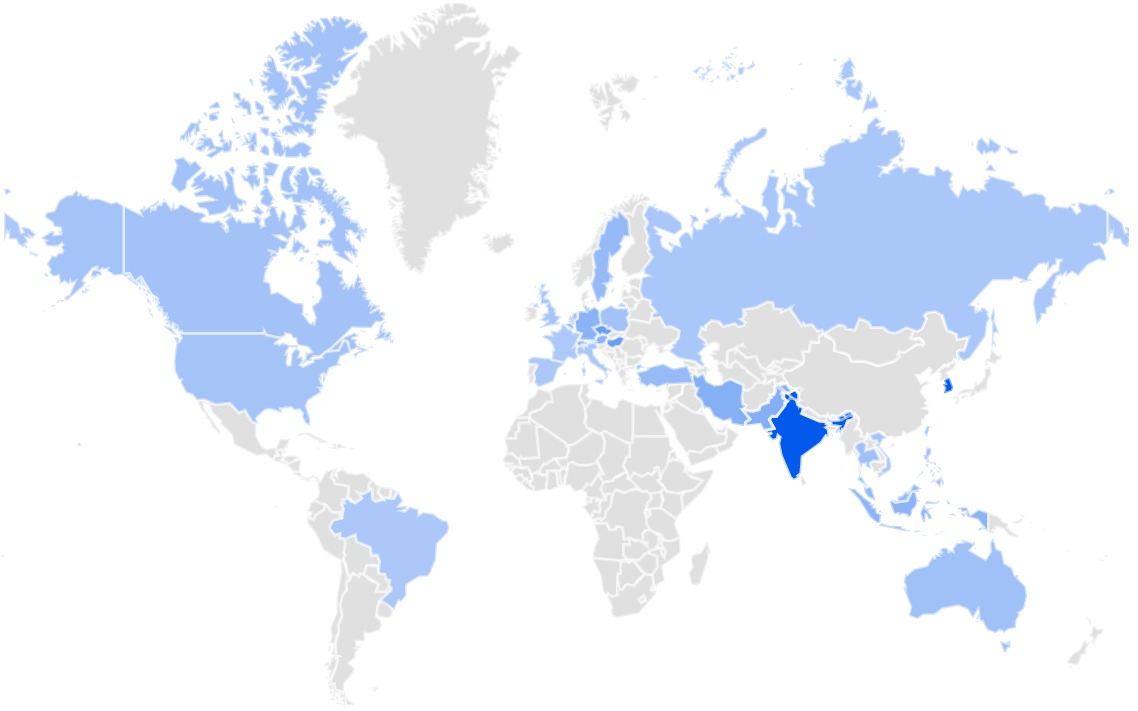
\includegraphics[width=.8\textwidth]{GoogleTrends_Map}
  \caption[Meiste Google-Suchanfragen seit 2004, anteilig nach Nation]{Meiste Google-Suchanfragen seit 2004, anteilig nach Nation (Quelle: Google Trends, Suchbegriff: \glqq{}bldc motor\grqq{})}
  \label{fig:Karte}
\end{figure}

Insbesondere der Aufstieg der Elektromobilität und der sich entwickelnden Industrie von E-Bikes und anderen akkubetriebenen Fortbewegungsmitteln dürfte seine Popularität positiv beeinflussen. Es ist anzunehmen, dass durch weitere technische Entwicklungen --- besonders dem entwickeln von kostensparenden Möglichkeiten und einfacherer Steuerungstechnik --- der bürstenbehaftete Gleichstrommotor immer weiter in den Hintergrund gedrängt und dessen Platz in immer mehr Sektoren vom BLDC-Motor besetzt wird.

%%% Local Variables:
%%% mode: latex
%%% TeX-master: "BLDC"
%%% End:
